\documentclass{rapportCS}
\usepackage{lipsum}
\usepackage{pdfpages}
\usepackage{tikz}
\usepackage{microtype}
\usepackage[T1]{fontenc}
\usepackage{txfonts}
\usepackage{enumitem}
\usepackage[utf8]{inputenc}
\usepackage[acronym, toc]{glossaries}
\usepackage{multicol}
\makeglossaries

\renewcommand{\labelitemi}{$\alpha$}

%------------- Acronymes --------------
\newacronym{SMOI}{S.M.O.I}{: Société Montage Océan Indien, créer le 1er Septembre 2001 sous le nom de \textit{travaux de maçonnerie général} puis transféré à un autre établissement le 1er Octobre 2005 sous le nom de \textit{SMOI} et enfin transféré à l'établissement dans lequel j'ai réalisé mon stage toujours sous le nom de \textit{SMOI} le 2 Novembre 2016. C'est une entreprise du secteur du bâtiment et elle faisait partie du groupe Solution BTP O.I. qui aujourd'hui est la société \textit{SMOI-XL location} suite à la fusion des entreprises du groupe}
\newacronym{AMOI}{A.M.O.I}{: Atelier Métallique Océan Indien, l'atelier de construction rattaché à la société SMOI}
\newacronym{DU}{D.U.}{: Document Unique d'évaluation des risque professionnel, est un document dans lequel est consigné le résultat de l'évaluation des risques pour la santé et la sécurité auxquels peuvent être exposés les salariés}

%----------- Crédits -------------------
% Template de rapport pour l'INSA Rennes basé sur le template "Template Stage Master IA - Université Le Mans" créé par Marie Tahon en 2023. 
% Thanks for Template Stage Master IA - Université Le Mans, By Marie Tahon (2023) that was the base for the creation of this template for INSA Rennes activity reports.
% Modifications apportées par Mateo Pena Campos en 2023 pour l'adapter au rapport de stage de l'INSA Centre Val de Loire.

\title{Rapport Stage ouvrier INSA 1A} 
\begin{document}

%----------- Informations du rapport ---------
%\titreligneun{\uppercase{Titre duZ }}
%\titrelignedeux{\uppercase{Document}}% Titre du document
%\soustitre{Rapport de Projet de Fin d'Études} % Sous-titre du document pour mentionné le type de document
%\numeroordre{Numéro d'ordre du PFE}
\departement{MIC} % Département pau sein de l'INSA
%\logoentreprise{
\includegraphics[scale=0.15]{logos/company_logo.png}} % Logo de l'entreprise pour inclure dans les marges du rapport, ajuster l'échelle selon la taille du logo.




%----------- Initialisation -------------------
\fairemarges % Afficher les marges
\fairecouverture % Créer la 1ère de couverture


%------------ Remerciements ----------------
\newpage
\vspace*{\stretch{1}}
\thispagestyle{empty} % Exclure cette page des marges et des numéros
\section*{Remerciements}
Je voudrais remercier ceux qui ont contribués à la bonne réalisation de ce stage: \newline
\begin{itemize}[label=$\bullet$] %
    \item G.VELECHY, le gérant de la société \acrshort{SMOI}* qui a accepté ma candidature dans son entreprise me permettant ainsi de découvrir l'organisation et le fonctionnement d'une entreprise.
    \item X.PAYET, mon tuteur de stage qui, m'a accompagné durant mon stage, et m'a ainsi permis d'apprendre et découvrir le travail ouvrier à travers les métiers de l'atelier.
\end{itemize}
\vspace*{\stretch{1}}


%------------ Table des matières ----------------
\newpage
\setcounter{tocdepth}{2} % Profondeur de la TOC
\thispagestyle{empty}
\tabledematieres % Créer la table de matières


%------------ Corps du rapport ----------------
%4+3+3+(1+4)=15

%------------ Introduction ----------------
\rhead{\nouppercase{\leftmark}}
\pagenumbering{arabic} % Commencer la numérotation des pages
\vspace*{\stretch{1}}
\setcounter{secnumdepth}{0}
\begin{center}
    \section{Introduction}
\end{center}
J'ai réalisé ce stage en fin de première année à l'INSA de Toulouse, dans le cadre de l'un de mes enseignements en tant qu'élève-ingénieur. L'objectif de celui-ci était de me permettre de découvrir le monde de l'entreprise à travers une expérience du travail ouvrier. Ce stage de quatre semaines en entreprise s'est déroulé lors de l'été 2023, du 10 Juillet au 8 Août dans l'atelier de l'entreprise de construction métallique \acrshort{SMOI}*.\par

J'ai alors été supervisé par X.PAYET, le responsable de l'atelier. Et j'ai réalisé, dans ce secteur de la construction métallique, la fabrication de charpentes à travers de la découpe, de la lecture de plan...\newline

Avant de réaliser ce stage, je savais que cette entreprise était une S.A.R.L, travaillant dans le secteur de la construction métallique et que celle-ci suivait actuellement un plan de redressement. J'ai alors choisi cette entreprise de part son secteur d'activité mettant directement en pratique toute la théorie que j'apprends, mais aussi parce que celle-ci est une moyenne entreprise me permettant ainsi de pouvoir observer l'intégralité du fonctionnement de l'entreprise.\par

J'espérais par ce stage pouvoir découvrir comment était créer les charpentes métalliques mais aussi toute la théorie autour du fonctionnement des machines et de la lecture de plans. Je voulais donc pouvoir découvrir et apprendre plus sur les acquis que j'avais déjà et de pouvoir me forger une opinion sur ce métier dans l'atelier dont j'avais une appréhension par comparaison avec les cours de technique de l'ingénieur que j'avais eu en première année.\newline

Cependant la recherche de ce stage ne s'est pas passée sans difficulté. En effet, au départ je n'avais envoyé aucun e-mail à cette entreprise et ne connaissais même pas son existence. Je n'ai à la suite de mes recherches et envoi de CV reçu que des réponse négative, me permettant ainsi de découvrir la difficulté qu'est la recherche de stage et/ou d'emplois dans le milieux professionnel. J'avais alors comme contrainte de trouver un stage ouvrier et comme objectif personnel de trouver un stage me permettant de pouvoir appliquer toute la théorie apprise lors de mes études.\newline

Dans un premier temps, je vais présenter l'entreprise dans laquelle j'ai réalisé mon stage, puis détailler les tâches réalisées, et enfin je terminerais par une analyse de l'entreprise à travers mon activité, rôle de stagiaire et ressenti dans celle-ci.

 
\vspace*{\stretch{1}}


%------------- Développement ----------------
\setcounter{secnumdepth}{1}


%------------- partie 1 -----------------
\newpage
\begin{center}
    \section{S.M.O.I, une entreprise dans le secteur du bâtiment}
\end{center}

\subsection{Information général}
%\textbf{- coordonnée forme juridique et appartenance à un groupe, explication du gérant(qui et création de l'entreprise, choix de celle-ci)}

La société SMOI, d'un capital de 850000 euros, est installée sur l'île de la Réunion aux 120 route des sable - local 5 zone industriel des sable - 97427 l'Etang-Salé France, et est une SARL, créer le 2 Novembre 2016 à la suite de la cloturation d'établissements secondaires (d'abord le 1 Octobre 2005 puis le 02 Novembre 2016). Cette entreprise se situe dans le secteur du bâtiment comme principal activité la construction de charpentes métalliques. Elle fait partie du groupe Solution BTP O.I.\footnote{Groupe d'entreprise situé dans le secteur du bâtiment, fondé par M. VELETCHY le 6 Mars 2023 sous le nom SMOI-XL location et comprenant les entreprise SMOI, AMOI, TMOI, XL location, entreprise VELETCHY \& FRERES} \newline
Les locaux sont composé de deux partie, la partie atelier (où sont fabriquer les charpente) et la partie bureau (où sont organiser les réunion d'information sur le projet et dessiner les plans).\newline

Le gérant actuel de cette société est M.VELETCHY. Il est également le dirigeant de plusieurs autres entreprises étant dans des secteurs d'activités proches tel que le prêt de matériels de chantier, de véhicule de chantier, de transport de marchandise etc.



\subsection{SMOI aujourd'hui, qui en sont les principaux acteurs ?}
%\textbf{- organisation général de l'entreprise (service de l'atelier, dessin, RH, compta) Nombre de salariés et qualification, organisation du travail, production, fournisseur, clientèle, concurrence}

Cette entreprise est organisée en deux parties comme dit précédemment, la partie atelier et la partie bureau ou l'on retrouve plusieurs services avec un service dédié à la réalisation des plans des différents projets en fonction du cahier des charges, un service ressource humaine et un service comptabilité.\newline
Elle est spécialisée dans la construction de charpente métallique mais aussi de gros œuvre\footnote{cf lexique p14}. Ayant pour principaux fournisseurs Micab, Kdi Davum et Ravate pro( tous trois fournisseurs de matériaux de construction et équipement). Et étant en concurrence directe avec de nombreuses autres entreprises tel que GTOI\footnote{Les grands travaux de l'océan Indien}, ou encore SARL Freres Lebon...\newline
Cette entreprise de 25 salariés vise principalement des particuliers avec par exemple la création d'une passerelle pour un cabinet de médecin, mais celle-ci intervient également sur de plus gros chantiers.



\subsection{Les politique d'hygiène et de sécurité dans l'entreprise}
%\textbf{- parler du qcm et faire ref à l'annexe}

Cette entreprise étant accès sur la construction de charpente métallique, présente de nombreux risque au niveau de la sécurité de ses salariés, il y a alors des politique qui sont mis en place ainsi qu'un certain nombre de réglementation à respecter afin de pouvoir entrer dans l'atelier (port obligatoire de protection visuelle, auditive, gants, tenu de travaille ininflammable, chaussure de chantier et casque de protection), des politiques et nouvelle norme de sécurité sont régulièrement mis en place, lors de réunion annuelle (avec la modification du Document Unique) visant à ré-évaluer les risque encouru par les employés lors des mission qui leur sont attribués, en fonction du nouveau matériel à acquérir ou non mais aussi en fonction des nouvelle tâche demandée dont les risque pourrait ne pas encore figurer dans le document et dont les mesure de sécurité ne serait alors pas encore prescrite.\newline
Un moyen de prévention cependant trop peu contrôlé, en effet il n'y a aucun suivi de la bonne réalisation et suivit de ce programme d'action mis en place ni de CSE\footnote{Comité sociale économique, l'anciennement Comité Hygiène et Sécurité des conditions de travail}. Il y a cependant des vérification régulière qui sont faite sur le matériel tel que les véhicule de chantier ou filet de protection.\footnote{cf annexe 1}



\subsection{SMOI, une entreprise engagé dans un esprit socio-écologique}
%\textbf{- parler du qcm et faire ref à l'annexe}

Malgré le fait que SMOI ne possède pas de service lié aux enjeux socio-écologique, celle-ci met en place des mesure afin de réduire son empreinte écologique et de préserver l'environnement, avec la présence d'un tri des matière première usé lors de la fabrication ainsi qu'un projet de mise en place d'une fosse hydrocarbure pour récupérer l'huile utilisé. Une partie de cet engagement se retrouve également dans une politique d'hygiène mise en place, qui est le nettoyage de l'atelier tous les vendredi soir, faisant le tri des métaux usés et un nettoyage méticuleux des sols tout en essayant au maximum de préserver l'environnement par ces actions. \newline

SMOI fait également appel à d'autres prestataires extérieurs afin de pouvoir faire le point sur ces conditions écologiques et enjeux importants et de mettre en place des solutions et méthodes. Et malgré l'absence de politique de réduction des émissions de gaz à effet de serre, il y a la présence de réunions chaque trimestre visant à faire le point cette fois-ci en interne sur les politique réaliser, la suivi de ces actions et une réflexion sur la possible mise en place d'autres.\footnote{cf annexe 3}



\subsection{Une entreprise qui cependant a de nombreuse difficultés}
%\textbf{- finance, plan de redressement}

La société SMOI est cependant depuis 2016 en difficulté financière avec une baisse de son chiffre d'affaires passant de 7.35M en 2016 à 2.38M en 2022 comme le montre ce graphique ci-dessous \ref{fig:CA_SMOI}.
\begin{figure}[h!]
    \centering
    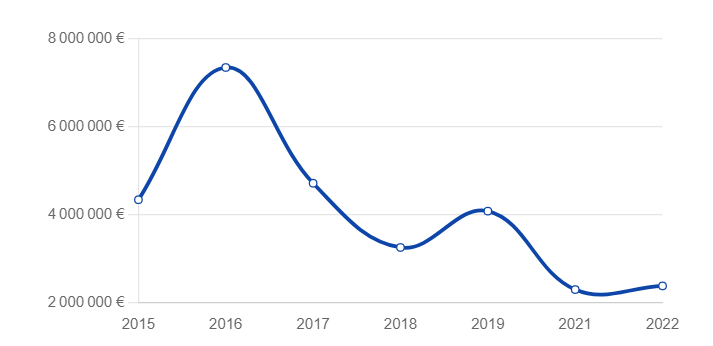
\includegraphics[width=0.75\textwidth]{figures/CA_SMOI.png}
    \caption{Évolution du chiffre d'affaire de la société SMOI de 2015 à 2022}
    \label{fig:CA_SMOI}
\end{figure}\newpage
Des difficultés se ressentent dans la quasi-totalité des entreprises du groupe \textit{Solution BTP O.I.} visible par l'évolution des résultats net du groupe. \ref{fig:résultat_solBTP}
\begin{figure}[h!]
    \centering
    \includegraphics[width=0.75\linewidth]{figures/résultat_solBTP.png}
    \caption{Évolution des résultats net du groupe Solution BTP O.I.}
    \label{fig:résultat_solBTP}
\end{figure}\newline
Il a donc été pris comme décision en Juillet/Août 2023 (donc durant ma période de stage) de dissoudre les société du groupe \textit{Solution BTP O.I.} et de transmettre leur capital social à l'entreprise \textit{Solution BTP O.I.} et ainsi de provoquer la fusion de toutes les entreprises en une seule afin de réduire les charges appliquées à celles-ci et permettre de relancer l'activité. En effet, depuis le 10 février 2022 et jusqu'au 21 Mars 2023 la société SMOI avait demander un plan de redressement judiciaire afin de pouvoir permettre d'avoir le temps de relancer l'activité, une procédure qui aboutira sur la fusion, cité précédemment, des entreprises du groupe en une \textit{Solution BTP O.I.} de nom commercial: \textsc{SMOI-XL location}.\footnote{cf annexe 4}\newline



\subsection{AMOI, l'atelier de SMOI.}
%\textbf{- moi dans l'entreprise, organigramme + technologie}

Cette entreprise, notamment sa partie atelier, \acrshort{AMOI}* qui grâce à sa proximité avec d'autre entreprise de prêt de matériel et véhicule de chantier, à accès à ceux-ci tel que des chariot élévateur et/ou des grues ainsi que des technologie de découpe plasma, des machine de pliage et de découpe de tôle et d'autre matière première métallique.\newline
J'ai réalisé mon stage dans ce secteur de l'entreprise chargée de la construction des charpentes suivant les plans réalisés par SMOI. Un atelier composé d'un responsable ayant les diplômes pour exercer et gérer les métiers dans l'atelier, de trois ouvriers de chantier, d'un chargé de la quincaillerie, et d'un chargé de la peinture et du revêtement des charpentes, organisé comme ci-contre dans cette organigramme.\ref{fig:organigram_AMOI}
\begin{figure}[h!]
    \centering
    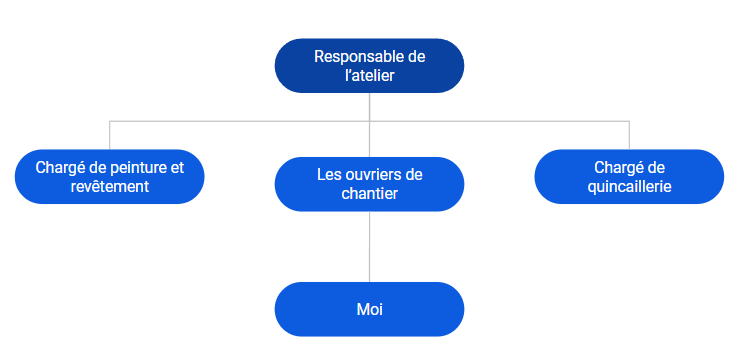
\includegraphics[width=1\linewidth]{figures/organigram_AMOI.png}
    \caption{Organigramme de AMOI}
    \label{fig:organigram_AMOI}
\end{figure} \newline


\subsubsection{Conclusion}
%résumer des information importante de cette première partie

Pour conclure cette partie, j'ai réalisé mon stage dans l'atelier de construction métallique de la société SMOI, une entreprise du secteur du bâtiment, qui faisait partie du groupe \textit{Solution BTP O.I.} et qui aujourd'hui est devenue la société \textit{SMOI-XL location} suite à un plan de redressement et la fusion de toutes les entreprises du groupe \textit{Solution BTP O.I.}. De plus, j'ai pu constater que cette entreprise avait des normes de sécurité et revue régulièrement en prenant en compte les missions données et qu'elle prenait également en compte les enjeux socio-écologiques actuels dans son fonctionnement.


%------------- partie 2 -----------------
\newpage
\begin{center}
    \section{Mon rôle en tant que stagiaire: fraisage, découpe, lecture de plan}
\end{center}

\subsection{AMOI: Atelier Métallique Océan Indien}
% 1, 2, 3, 6 et 7 (ne pas hésité à mettre des sous section)

\subsubsection{Place et fonction du service}% 1 et 2
L'atelier AMOI, à pour objectif la réalisation des structures (charpente métallique, gros œuvres, installation sur chantier...) dont les plans sont fournis par les dessinateur de SMOI. Ce service à donc pour fonction la réalisation physique des demandes des clients.

\subsubsection{Moyen matériel et humain du service}% 3 et 6
L'atelier est composé de six salariés, trois ouvriers de chantier, un responsable de l'atelier, un chargé de la quincaillerie et un chargé de la peinture et des revêtements. Il est alors séparer en cinq parties:
\begin{enumerate}
    \item L'entrepôt des matières première et/ou des produit en cours de transformation
    \item L'entrepôt des outils, corde, échelle, la quincaillerie
    \item Un espace dédié à la pose de peinture et de revêtement
    \item Un espace dédié aux machine, pour la découpe, la soudure, le pliage, la transformation des matière première
    \item Un espace dédié au vestiaire
\end{enumerate}
Les principaux matériaux transformés dans l'atelier sont le fer, l'aluminium, l'inox et la tôle. Il sont alors transformés à l'aide de différente machine tel que une machine à découpe plasma\footnote{cf lexique p14}, une plieuse \ref{fig:plasma_plie}, une fraiseuse\footnote{cf lexique p14}, une machine de scie à eau, une presse hydraulique mais également des outils tel que des perceuses magnétique, des foreuse portable et des ponceuse.
\begin{figure}[h!]
    \centering
    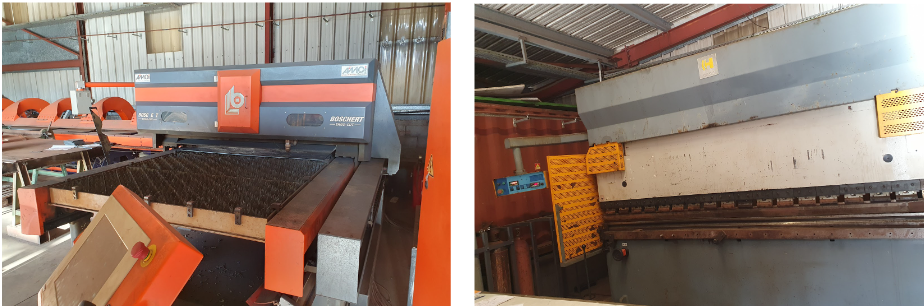
\includegraphics[width=1\linewidth]{figures/plasma_plie.png}
    \caption{Machine à découpe plasma \& Machine plieuse de tôles}
    \label{fig:plasma_plie}
\end{figure} \newpage
Étant donnée de cette équipe réduite, les communications en interne sont simplifiées. En effet, les interactions entre les autres services et l'atelier passe principalement par le responsable de l'atelier qui reçoit les dessinateurs pour faire le point sur les commandes avenir et les délais. De plus, comme l'équipe est réduite, l'organisation de réunion entre elle est peu compliquée et contraignante.\newline
En externe j'ai pu constater qu'il y avait des réunions avec les clients et que les fournitures passait principalement par commande téléphonique.\par

\subsubsection{Des dysfonctionnement matériel inquiétant}% 7
Cependant lors de mon stage l'entreprise a dû faire face à la panne de leur machine plieuse de tôles ralentissant alors fortement leur activité dans ce secteur durant presque plus d'un mois. Il y a tous au long de mon stage dans cette entreprise, eu la visite de réparation dans le but de réaliser les mise à jour nécessaire sur la machine et la remettre en état, cependant cela c'est avéré vain. Il a donc été pris la décision de remplacer la machine. Une opération délicate puisque nécessitant la venue d'une grue et le démantèlement d'une partie du toit de l'atelier.


\subsection{Mon activité de stagiaire}
% 4, 5 et 8 (une sous section pour chaque activité réalisé + une sous section général pour les info général)

Lors de mon stage j'ai travaillé de 8h à 12h puis de 13h à 16h du lundi au jeudi et de 8h à 12h le vendredi. Mes tâches étaient réparties en fonction de ce qui était disponible et des missions sur lesquelles l'atelier travaillait. Mais j'ai principalement réalisé des tâches de fraisages et lecture de plan de début de semaine et des tâches de nettoyage en fin de semaine.
\subsubsection{Fraisage}
La première et principale tâche que j'ai réalisée lors de mon stage était du fraisage, mais pour celle-ci on m'a expliqué le fonctionnement des machines (donc ici de la fraiseuse et des perceuses magnétiques). Je devais donc en suivant les cotations et norme imposée sur les plan et dessiner sur les barre de métal découper, percer des trou avec les bonne fraise, soit en utilisant une perceuse magnétique pour les barre de métals trop grosse et grande pour la fraiseuse, soit en utilisant la fraiseuse afin de réaliser des trou qui avait pour certain but d'être boulonné mais pour d'autre but de servir d'emplacement pour des vis. J'ai notamment réaliser le perçage de plaque servant à la réalisation d'un escalier, il fallait donc que j'utilise la fraiseuse avec une fraise spécifique de tel manière à percer précisément une plaque (sans pour autant la perforé entièrement) pour permettre le passage de vis à bois.
\subsubsection{gravure}
Après avoir perforé correctement les pièces métalliques, je me suis servi d'une machine à gravure par percussion afin de noter les référence de chacune des pièces (référence noté sur les schémas de coupes) pour pouvoir les entreposer en attendant la prochaine étape de leur transformation.
\subsubsection{Lecture de plan}
Une autre de mes tâche était la lecture de cotation sur les différents plan de coupes, assemblages\footnote{cf annexe 5} et pliages et de noter, dessiner avec précision sur les pièce considérer le marquage nécessaire pour la réalisation de pliage (notamment pour les tôles), le fraisage et la découpe. Une étape nécessitant une grande précision et dont le travail réalisé est systématiquement contrôlé avant toute autres actions de pliage ou de découpe.
\subsubsection{Découpe}
J'ai opéré deux type de découpe durant mon stage:
\begin{itemize}
    \item Une découpe plasma: On ne m'a pas appris le fonctionnement précis et l'utilisation du logiciel permettant le pilote de la machine, mais j'étais chargé de surveiller le fonctionnement de la machine qui avait quelques bugs et pour qui le programme devait être redémarer si cela arrivait. Je devais, à la suite du découpage, démouler les pièces des plaques découpées, les annoter de leurs références, les nettoyer en utilisant soit un burin, soit en utilisant une ponceuse puis percer les trous mal formés lors de la découpe et de les graver après soudure.
    \item Une découpe à l'eau: J'ai également reçu pour mission de réaliser des découpes précises de barres de métaux et/ou d'aluminium en utilisant une scie à eau. Je devais donc aller chercher les matières premières entreposées, les placer sur la machine en suivant les cotation du schéma de coupe et vérifier en fin de coupe la longueur si la longueur coupé était bien celle attendue.
\end{itemize}
\subsubsection{ponçage/meulage}
J'ai aussi réalisé du ponçage et du meulage, qui était pour mes mission, des mission de nettoyage des pièce intermédiaire, tel qu'avec une ponceuse, j'ai enlever les traces de la présence de point de soudure.
\subsubsection{pliage}
Une fois le remplacement de la machine de pliage effectué, j'ai pu non pas réalisé du pliage seul mais aider au maintien et placement des tôles pour leur pliage.
\subsubsection{montage}
Je suis également partie sur un chantier\footnote{cf annexe 6}, ici chez un particulier (un cabinet médical), dans lequel j'ai participé à l'installation d'une passerelle préalablement fabriquée dans l'atelier. J'ai donc participé à l'installation des piliers de celle-ci en forant les trous dans le sol pour y installer les vis allant dans les pieds des piliers. Je n'ai cependant, puisque n'ayant pas les habilitations nécessaires pour les travaux en hauteur, pas pu énormément participé quant à l'installation de la partie haute de la passerelle.\ref{fig:pillier_passerelle}
\begin{figure}[h!]
    \centering
    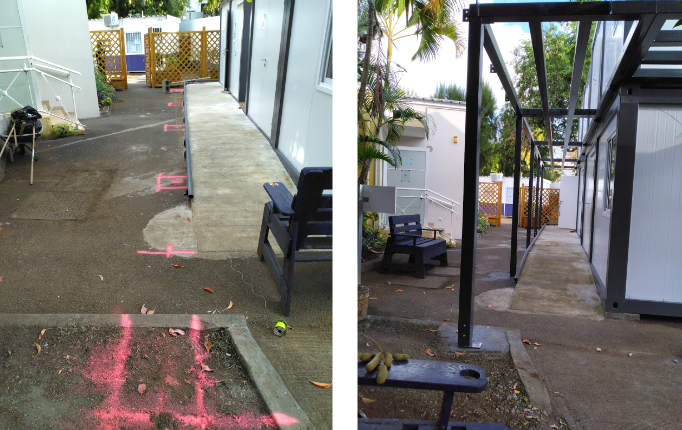
\includegraphics[width=1\linewidth]{figures/pillier_passerelle.png}
    \caption{photo de la passerelle avant et après installation des piliers}
    \label{fig:pillier_passerelle}
\end{figure}
\subsubsection{nettoyage}
La dernière tâche que j'ai réalisé à été de nettoyer, en passant le balais dans l'atelier, en triant les matières premières usées mais également en nettoyant les machine, notamment, la machine à découpe plasma avec l'aide du responsable de l'atelier.


\subsubsection{Conclusion}
%mini conclusion et résumé des info de la partie

Pour conclure cette partie, j'ai réalisé les principales tâche de la conception d'un produit à travers la fabrication des pièce intermédiaire pour l'assemblage, des activité qui chez moi ont suscité de l'intérêt avec des questionnement et recherche d'explication sur leur fonctionnement (des machine mais aussi des méthode de fabrication). Et cela malgré les péripéties survenu durant mon stage avec la panne d'une machine.


%------------- partie 3 -----------------
\newpage
\begin{center}
    \section{L'entreprise SMOI, une expérience unique}
\end{center}

\subsection{Un ressentis contraster}
% 1, 2 et 5

Lors de mon stage j'ai pu faire les frais d'un environnement de travail difficile, avec énormément de bruit d'un niveau sonore très élevé (normal pour un atelier de construction métallique) engendrant des difficultés de compréhension de ce qu'on essayais de me dire, mais il y avait aussi une forte exposition au soleil, augmentant d'autant plus la pénibilité des tâches à réaliser.\newline
Malgré cet environnement de travail difficile, l'ambiance de travail en elle-même au sein de l'entreprise est douce, chaleureuse et amicale. Ainsi même en cas de soucis ou de difficulté lié à la timidité ou en étant nouveau donc comme cela était mon cas, l'ambiance est incroyablement chaleureuse et celle-ci permet alors de tisser des liens et d'avoir un très bon relationnel. J'ai donc malgré ma timidité et difficulté à communiquer avec les autres immédiatement été rassuré.\newline

Cette ambiance de travail se reflétait également avec de bonnes conditions de sécurité avec des règles très strictes. Ce stage m'a alors permis de beaucoup apprendre sur comment était réalisé les charpentes des bâtiments, les étapes à suivre, leur but mais aussi le fonctionnement des machines. Et c'est cette partie même qui m'a le plus plu dans mon stage, avoir la possibilité d'en apprendre plus sur un sujet et de découvrir le fonctionnement des machines ainsi que des méthodes de fabrication et avoir ainsi l'expérience d'une application directe de la théorie apprise en classe.\newline
Mes activités me permettent ainsi d'avoir une connaissance plus large sur le domaine de la fabrication, les procédés utilisés, leur but et le fonctionnement des machines, provoquant alors un fort sentiment de satisfaction en regardant le travail qu'on a réalisé terminer et se rendre ainsi compte de tout ce qu'on peut vraiment faire soit même avec de la matière première et les bon outils.\newline

Dans l'entreprise j'ai réalisé des tâches de fraisage, découpe, gravure et polissage, j'ai donc en résumer réaliser les tâches de la préparation intermédiaire des matière première avant l'assemblage et la peinture de celle-ci. Des tâches qui dans cette société ne sont pas automatisées puisque chaque élément est fait sur mesure en fonction de critères des clients en particulier et non pas pour la grande distribution.\newline
J'occupais alors une place importante dans la chaîne de fabrication puisqu'étant placé à l'étape juste avant l'assemblage des pièces.



\subsection{un stage présentant des difficulté inattendu}
% 3 et 4

Avant d'effectuer mon stage j'avais quelque appréhension concernant le côté relationnel qui n'est pas mon point fort. J'ai ainsi rencontré comme je le craignais des difficulter à m'adapter à l'ambiance qui régnait ainsi qu'à développer le côté relationnelle. Cependant j'ai également dû faire face à un difficultés que je ne pensais pas arrivé qui était les difficultés de compréhension du au vocabulaire précis utiliser que je pensais connaître suffisamment avant d'avoir réaliser mon stage.\par
J'ai donc pour palier à ces difficultés, dans un premier temps au niveau relationnelle, forcé la conversation en essayant d'en apprendre plus sur les autres membre de l'atelier mais également en essayant d'en comprendre plus sur le fonctionnement des machine ainsi que sur la raison et l'utiliser de certain procédé et méthode de fabrication. En ce qui concerne les problème de compréhension je n'ai cependant pu totalement m'en débarrasser, puisque je ne pouvais pas voir l'entièreté du vocabulaire de l'atelier juste sur une ou deux mission réalisé, j'ai du apprendre tout au long de mon stage du nouveau vocabulaire au fil des jours et palier de manque de compréhension par des demande d'explication.



\subsection{une entreprise en pleine innovation}
% cf qcm annexe 2 + DU

J'ai pu constater lors de mon stage que la société SMOI était en constante évolution avec la présence d'une innovation qui est l'agrandissement de l'atelier et la mise en place d'un raille de transport permettant de transporter les matière première et celle de transition d'un bout à l'autre de l'atelier pour leur transformation, une innovation permettant d'accélérer et facilité la production (donc étant bénéfique pour les ouvriers) de part une plus grande mobilité et un plus grand espace de travail.\ref{fig:innovation}\newline
Une entreprise innovante mais qui tout de même à mon avis, après en avoir discuté avec le gérant, pourrait s'améliorer sur un autres point, ici plus accès sur la sécurité au travail avec le \acrshort{DU}* qui même s'il est revu chaque année en fonction des nouvelles missions et/ou du nouveau matériel à disposition, ne présente pas vraiment de suivi de la bonne réalisation des normes et précautions mis en place que cela soit par un service interne liée à la sécurité du travail ou par des prestataires externes.\footnote{cf annexe 1} \newline

Je suggérerais donc en voie d'une amélioration de leur système et politique de sécurité au travail, en vue notamment de cette innovation (agrandissement de l'atelier) qui va entraîner la naissance de nombreux autres risque pour la sécurité des travailleur, de soit mettre en place un secteur dédié à la rédaction de ce Document Unique ainsi qu'à sa communication et au contrôle de sa bonne suivit en interne ou encore de faire appel à un prestataire extérieur spécialisé dans ce domaine de la sécurité au travail afin de contrôler l'application de ces mesure et d'avoir un retour concret sur celle-ci pour les modification futur du DU.
\begin{figure}[h!]
    \centering
    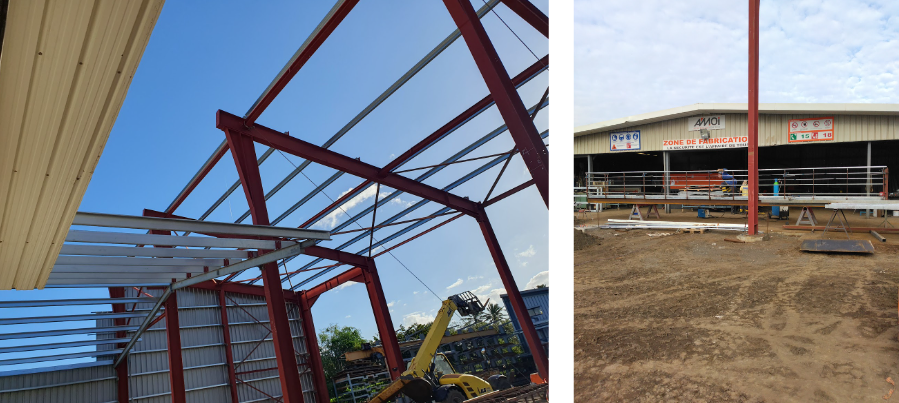
\includegraphics[width=1\linewidth]{figures/innovation.png}
    \caption{photo du projet d'innovation en cours}
    \label{fig:innovation}
\end{figure}



\subsubsection{Conclusion}
%mini conclusion et résumé des info de la partie

Pour conclure cette partie, la société SMOI est très accueillante, et présente de nombreux points positifs quant à la sécurité et sur l'innovation et sont amélioration, malgré la présence de quelque point négatif notamment au niveau du suivi du respect des mesure du DU. J'ai alors rencontré quelques difficultés qui se sont rapidement résolues par une implication relationnelle de ma part. Me permettant ici de mieux appréhender l'importance de chaque main, du relationnel mais aussi les réflexions autour de l'innovation et de la sécurité dans le monde de l'entreprise.


%------------- Commandes utiles ----------------
%\newpage
\section{Quelques commandes}
\subsection{Insertion de listes}
\textbf{Consignes du moodle INFO, à adapter selon le département :}
\newline
Le rapport comprend nécessairement des parties incontournables :
\begin{itemize}[label=$\bullet$] %
    \item Une \textbf{couverture} respectant le modèle unifié imposé (disponible au format .doc) et mentionnant votre numéro d'ordre (visible sur la liste des correspondants enseignants). 
    \item La mise en page du contenu de votre document reste libre.
    \item Si vous rédigez en LaTeX vous pouvez rajouter la couverture (après conversion en .pdf du document obtenu à partir du fichier .doc) :
         \begin{enumerate}
            \item page 1 : Couverture avec le titre
            \item page 2-3 : ADA
            \item contenu édité en LaTeX
            \item page N-1 : double résumé 
            \item page N : dernière couverture (avec le logo INSA)
        \end{enumerate}
        
    \item Une partie introductive décrivant succinctement l'entreprise d'accueil et le sujet du stage (de quelques pages tout au plus).
    \item Une partie principale décrivant le travail réalisé pendant le stage. Il est utile de structurer ce travail, de hiérarchiser l'importance de chaque axe (si plusieurs) afin de mieux mettre en évidence les aspects techniques complexes, non triviaux (i.e., qui prouvent qu'il s'agit d'un travail de niveau M2), sans toutefois rentrer dans tous les détails techniques des aspects moins importants. La présentation doit être « didactique » : elle doit être compréhensible par un informaticien non spécialiste du domaine d'application de votre stage. Elle doit mettre en évidence le travail que vous avez effectivement réalisé.
    \item Une partie conclusion montrant d'une part, les apports de vos travaux pour l'entreprise et d'autre part, les enseignements que vous avez personnellement retirés de ce stage.
    \item Une partie annexe donnant un planning du stage en semaines indiquant la durée des différentes phases (étude, analyse fonctionnelle, codage, tests...).
    \item Une partie bibliographique comparant vos travaux avec ceux déjà effectués sera parfois nécessaire dans le document.
    \item Un double résumé français et anglais (une page au total, en 3e de couverture, c-à-d l'avant-dernière page du rapport).
        \begin{itemize}[label=$\diamond$]
            \item La consigne associée à ce résumé bilingue est d'être didactique et accessible à un non informaticien, pour par exemple être compris d'un jeune étudiant intéressé par le département informatique.
        \end{itemize}
\end{itemize}
Ce rapport doit être rédigé en français ou en anglais et ne pas dépasser 30 à 40 pages pour les parties mentionnées ci-dessus. Il peut être associé à une annexe technique comportant autant de documents que vous souhaitez absolument adjoindre au rapport final, mais dont la lecture doit demeurer facultative.
\subsection{Insertion de figures}
%------ Pour insérer et citer une image centralisée -----
% Le premier argument est le chemin pour la photo
% Le deuxième est la hauteur de la photo
% Le troisième la légende
% Le quatrième le label
Ici, je cite la figure \ref{fig:my_label} dans le texte.
\begin{figure}[h!]
    \centering
    
\includegraphics[width=0.8\textwidth]{figures/vincent-brunie.jpg}
    \caption{Mettre une légende explicite à votre figure, ici M. Brunie Directeur de l'INSA Rennes.}
    \label{fig:my_label}
\end{figure}

\subsection{Insertion d'équation}
%------- Pour insérer et citer une équation --------------

\begin{equation} \label{eq: exemple}
\sum_{\rho=1}^{\infty} (\rho . \Delta) = 42, \Delta \in \mathbf{R}
\end{equation}

L'équation \ref{eq: exemple} est citée ici. 

\subsection{Insertion d'une référence bibliographique}
Les références (articles scientifiques, articles de journaux, blogs, pages web) doivent être mentionnées dans le texte par une balise \cite{maref} et fait le lien avec la citation incluse dans la bibliographie.

\subsection{Ajout au glossaire}

\acrshort{abc}* voilà comment on ajoute un acronyme au texte.




%------------ Conclusion ----------------
\newpage
\vspace*{\stretch{1}}

\setcounter{secnumdepth}{0}
\begin{center}
    \section{Conclusion}
\end{center}
En conclusion, avant de réaliser mon stage chez la société SMOI, j'avais de nombreuses appréhensions mais aussi attente en ce qui concerne mon apprentissage et ma compréhension des métier de l'atelier et en général, d'une application directe de mes apprentissage théorique.\par
En effet, en ce qui concerne l'aspect relationnel, la prise de décision, l'organisation, les réflexions autour de la sécurité, de l'innovation mais aussi tour de l'impact écologique, mes attentes ont été largement dépassées et je ne pouvais espérer en apprendre autant sur le sujet. Ce stage m'a permis également de pouvoir développer mes connaissance scientifique et d'être satisfait au niveau de la découverte des application des sujet théorique que sont les science de l'ingénieur\newline

J'ai alors participé à ce stage en tant qu'observateur, avec l'apprentissage des notions citées précédemment, mais aussi en tant qu'acteur de celui-ci étant au centre de la chaîne de production des produits de l'entreprise SMOI. J'en aie alors tirer des leçon pratique sur l'organisation d'une équipe (les délais, relation client, répartition des tâches...); me permettant alors d'envisager une perspective d'avenir plus clair, avec ce stage ayant pour place d'une expérience bénéfique mais également d'un exemple sur lequel je peux me baser pour la poursuite de mes étude et la recherche de mon orientation future.
\vspace*{\stretch{1}}


%-------------- Bibliographie -----------------------
%\newpage
%\rhead{\nouppercase{\leftmark}}
%\bibliographystyle{apalike} % définit le style de bibliographie, ici APA
%\bibliography{references} % ajoute la bibliographie basée sur le %fichier references.bib


%--------------- Glossaire & Acronymes -------------
\newpage
\vspace*{\stretch{1}}

\printglossary[type=\acronymtype]
\label{sec:acronymes}
\setcounter{secnumdepth}{0}
\section{Lexique}
\begin{itemize}
    \item \textbf{Gros œuvre}: pour une maison représente l'ensemble des travaux participant à la stabilité et à la solidité du logement tel que la réalisation des fondations d'une maison. Il s'agit de travaux permettant à la construction de résister à son propre poids et aux agressions extérieures.
    \item \textbf{découpe plasma}: Le découpage plasma est un procédé de découpage par fusion localisée, dans lequel un jet de gaz ou d’air comprimé vient faire fondre instantanément le métal porté à une température de fusion. Une température proche de 18000 °C est alors générée par l'arc électrique créé entre la torche (embout de la machine pour la découpe) et la plaque de métal.
    \item \textbf{fraisage}: Procédé dans lequel un outil enlève de la matière par un mouvement rotatif. Comme pour le perçage, il est possible d'utiliser un large éventail d'outils de différents diamètres et de différentes duretés.
\end{itemize}
\vspace*{\stretch{1}}


%--------------- Table des illustrations -------------
\newpage
\vspace*{\stretch{1}}
\begin{center}
    \section{Table des illustrations}
\end{center}
\begin{itemize}
    \item figure 1: Évolution du chiffre d'affaire de la société SMOI de 2015 à 2022 / \href{https://www.pappers.fr/entreprise/smoi-societe-montage-ocean-indien-439139668}{pappers.fr} / page 3
    \item figure 2: Évolution des résultats net du groupe Solution BTP O.I. / \href{https://www.pappers.fr/entreprise/solutions-btp-oi-819693706}{pappers.fr} / page 4
    \item figure 3: Organigramme de AMOI / organigramme personnel / page 5
    \item figure 4: Machine à découpe plasma \& Machine plieuse de tôles / photo personnel / page 6
    \item figure 5: photo de la passerelle avant et après installation des pilliers / photo personnel / page 9
    \item figure 6: photo du projet d'innovation en cours / photo personnel /page 11
\end{itemize}
\vspace*{\stretch{1}}


%--------------- Annexes -------------
\newpage
\vspace*{\stretch{1}}
\begin{center}
    \section{Table des annexes}
\end{center}

\begin{itemize}
    \item Annexe 1: Sensibilisation à l'Hygiène et à la Sécurité / page 1
    \item Annexe 2: Sensibilisation à l'innovation en entreprise / page 3
    \item Annexe 3: Les enjeux socio-éconologique dans l'entreprise / page 5
    \item Annexe 4: Extrait de l'acte de dissolution et de fusion de SMOI à Solution BTP O.I. / page 7
    \item Annexe 5: Schéma de plan de coupe d'un assemblage / page 11
    \item Annexe 6: photo de la passerelle du chantier d'un cabinet médical / page 12
\end{itemize}
\vspace*{\stretch{1}}
\annexeObli
\AnnexeFacul

\end{document}

